\subsection{Simulación de tormentas}

El segundo sistema natural es el movimiento de las tormentas. A diferencia del fuego, que solo avanza sobre el terreno que no se ha quemado, una tormenta se desplaza con el viento, crece, se debilita y puede aparecer en zonas donde antes no llovía.

Este experimento se alimenta del conjunto de datos SEVIR (\textit{Storm EVent ImagRy}) \cite{veillette2020sevir}, que reúne más de 10,000 eventos meteorológicos registrados en los Estados Unidos entre 2017 y 2019. Cada evento cubre una zona de $384 \times 384$ km durante 4 horas y contiene imágenes de radar y de satélite. De todas ellas, solo se utiliza el VIL (\textit{vertically integrated liquid}), que mide la cantidad de agua líquida en la columna de aire sobre cada kilómetro cuadrado: un valor alto indica lluvia intensa o granizo. Cada evento tiene 49 imágenes de $384 \times 384$ píxeles (1 km por píxel), una cada 5 minutos.

Del conjunto completo se descargaron los 19,093 eventos que tienen VIL completo: 3,536 corresponden a tormentas registradas en la base de datos de eventos severos y 15,557 a eventos aleatorios. En este experimento solo se utilizan las tormentas.

\subsubsection{Preprocesamiento de los datos}

Para la limpieza del conjunto de datos, se procedió de la siguiente manera:

\begin{enumerate}
	\item Escalado de la evolución: Cada imagen se reduce de $384 \times 384$ a $96 \times 96$ células promediando bloques de $4 \times 4$ píxeles, por lo que cada célula representa 4 km. Con esta escala, una tormenta avanza alrededor de una célula por paso, lo que permite capturar su movimiento con una vecindad pequeña.

	\item Discretización: Se utilizan los 6 umbrales de VIL que proponen los autores de SEVIR para evaluar pronósticos (16, 74, 133, 160, 181 y 219, en la escala de 0 a 255 del conjunto de datos), lo que da 7 estados: el estado 0 indica que no hay lluvia y el estado 6, la lluvia más intensa (tabla \ref{tab:sevir_estados}). En adelante, se considera que una célula tiene tormenta si su estado es 2 o mayor, es decir, si su VIL es de al menos 74. La figura \ref{fig:sevir_preprocesamiento} muestra el resultado de ambos pasos.

	\item Selección de eventos: Para que la red no aprenda que las tormentas aparecen de la nada, se eligen al azar eventos en los que al menos el 2\% de las células tienen tormenta desde la primera imagen. El conjunto de entrenamiento tiene 40 tormentas de 2018 y el de prueba, 20 tormentas de 2019, por lo que la red se prueba con tormentas de otro año que nunca vio.
\end{enumerate}

\begin{table}[htbp]
	\centering
	\footnotesize
	\begin{tabular}{cccc}
		\toprule
		& & \textbf{Porcentaje en} & \textbf{Porcentaje en} \\
		\textbf{Estado} & \textbf{VIL} & \textbf{entrenamiento} & \textbf{prueba} \\ \midrule
		0 & 0--16 & 70.76 & 68.01 \\
		1 & 16--74 & 12.63 & 15.19 \\
		2 & 74--133 & 11.33 & 12.41 \\
		3 & 133--160 & 3.15 & 2.52 \\
		4 & 160--181 & 1.09 & 0.90 \\
		5 & 181--219 & 0.87 & 0.75 \\
		6 & 219--255 & 0.17 & 0.21 \\
		\bottomrule
	\end{tabular}
	\caption{Estados de SEVIR según el VIL de cada célula y su porcentaje en los conjuntos de entrenamiento (40 tormentas de 2018) y prueba (20 tormentas de 2019).}
	\label{tab:sevir_estados}
\end{table}

\definecolor{sevir0}{HTML}{F2F2F2}\definecolor{sevir1}{HTML}{9BE39B}\definecolor{sevir2}{HTML}{2E9E3A}
\definecolor{sevir3}{HTML}{F5D90A}\definecolor{sevir4}{HTML}{F28C1E}\definecolor{sevir5}{HTML}{D7191C}
\definecolor{sevir6}{HTML}{B10DC9}
\newcommand{\estadosevir}[2][black]{\fcolorbox{gray}{sevir#2}{\makebox[1.1em]{\textcolor{#1}{#2}}}}
\newcommand{\leyendasevir}{%
	\par\medskip
	{\footnotesize\setlength{\fboxsep}{1pt}%
	Estado: \estadosevir{0}\estadosevir{1}\estadosevir[white]{2}\estadosevir{3}\estadosevir{4}%
	\estadosevir[white]{5}\estadosevir[white]{6}\par}}

\begin{figure}[htbp]
	\centering
	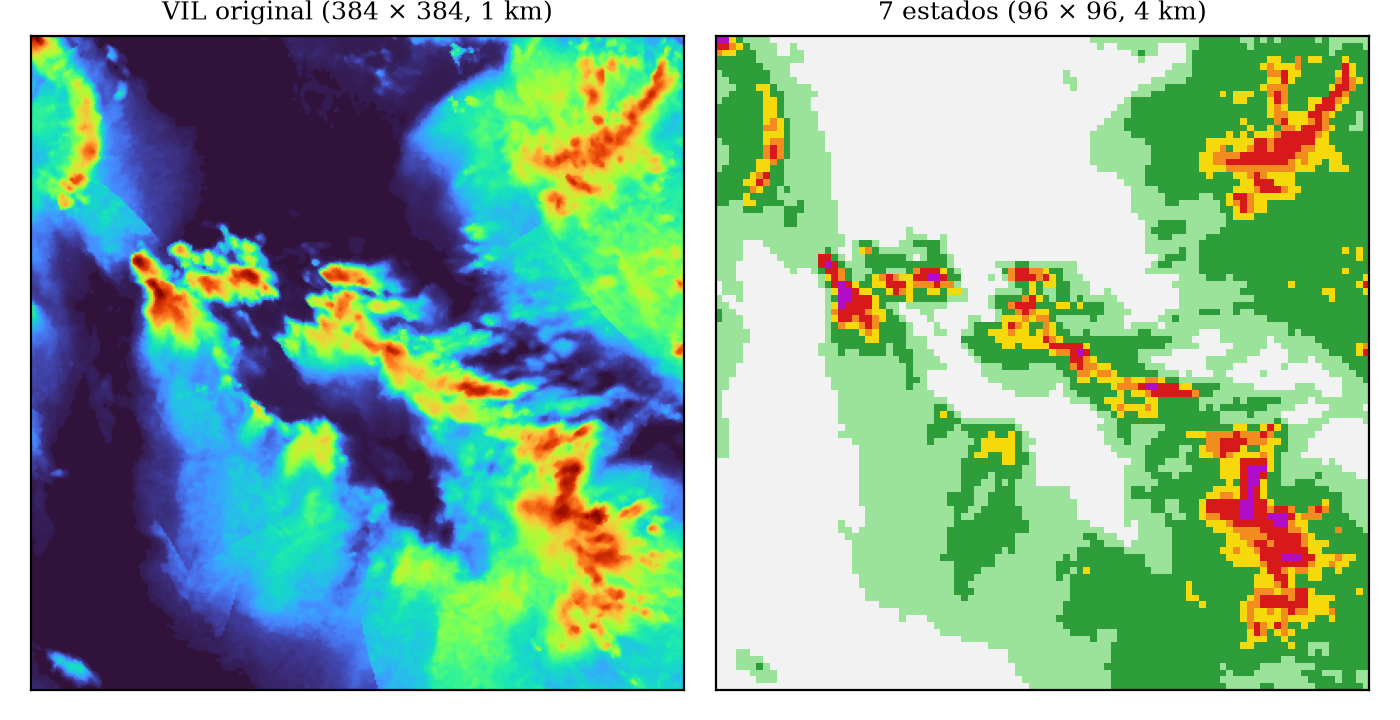
\includegraphics[width=0.8\linewidth]{img/experimentacion/naturales/SEVIR/preprocesamiento.png}
	\leyendasevir
	\caption{Primera imagen de una tormenta del conjunto de prueba (27 de mayo de 2019): VIL original y sus 7 estados después del escalado.}
	\label{fig:sevir_preprocesamiento}
\end{figure}

\subsubsection{Capacidad de replicación}

Se probaron 4 configuraciones: vecindad de $5 \times 5$ (25 vecinos) o de $9 \times 9$ (81 vecinos), y capas ocultas de 2:32:ReLU o 3:64:ReLU, con capa de salida 7:Linear. Todas usan \textit{one-hot}, por lo que la capa de entrada tiene $25 \times 7 = 175$ entradas con la vecindad de $5 \times 5$ y $81 \times 7 = 567$ con la de $9 \times 9$. Todas se entrenaron durante 30 épocas con entropía cruzada como función de pérdida, una tasa de aprendizaje inicial de 0.001 con reducción exponencial hasta 0.00001, un tamaño del lote de 8,192, frontera abierta y semilla aleatoria 42. El conjunto de entrenamiento tiene 17,694,720 muestras (40 tormentas, 48 pasos y $96 \times 96$ células); a diferencia de FLAME~3, cada entrenamiento tardó menos de un minuto.

Al igual que en FLAME~3, las redes se comparan con la predicción sin cambio, que supone que la siguiente imagen es igual a la actual. Se usan dos medidas:

\begin{enumerate}
	\item La exactitud es el porcentaje de células con el estado correcto.
	\item El área con tormenta indica qué tanto se parecen las células con tormenta (estado 2 o mayor) de la simulación a las reales. Un valor de 100\% significa que son idénticas.
\end{enumerate}

Ambas medidas se calculan de dos formas: prediciendo un solo paso desde cada imagen real de las 20 tormentas de prueba, y en la simulación libre, en la que la red parte de la primera imagen y evoluciona sola con sus propias predicciones durante 4 horas.

La tabla \ref{tab:sevir_resultados} muestra los resultados. Las 4 configuraciones superan a la predicción sin cambio en todas las medidas, aunque por poco: en un paso aciertan entre el 89.30 y el 89.37\% de las células, contra el 87.64\% de la predicción sin cambio, y en la simulación libre su área con tormenta se parece a la real entre un 4 y un 5\% más que la de la predicción sin cambio a los 30, 60 y 120 minutos. Las diferencias entre configuraciones son muy pequeñas: aumentar la vecindad o el tamaño de la red reduce la pérdida, pero no mejora la simulación libre.

\begin{table}[htbp]
	\centering
	\footnotesize
	\setlength{\tabcolsep}{4pt}
	\begin{tabular}{@{}cccccccc@{}}
		\toprule
		& & & & & \multicolumn{3}{c}{\textbf{Área con tormenta en}} \\
		& & & \multicolumn{2}{c}{\textbf{Un paso}} & \multicolumn{3}{c}{\textbf{la simulación libre}} \\
		\cmidrule(lr){4-5} \cmidrule(l){6-8}
		& & & & \textbf{Área con} & & & \\
		\textbf{Vecindad} & \textbf{Capas} & \textbf{Pérdida} & \textbf{Exactitud} & \textbf{tormenta} & \textbf{30 min} & \textbf{60 min} & \textbf{120 min} \\ \midrule
		\multicolumn{3}{c}{Predicción sin cambio} & 87.64\% & 76.93\% & 45.52\% & 32.43\% & 19.93\% \\ \midrule
		\multirow{2}{*}{$5 \times 5$} & 2:32 & 0.2266 & 89.30\% & 79.83\% & 50.24\% & 37.00\% & 23.77\% \\
		& 3:64 & 0.2245 & 89.31\% & 79.90\% & 50.22\% & 36.86\% & 23.38\% \\
		\multirow{2}{*}{$9 \times 9$} & 2:32 & 0.2226 & 89.35\% & 79.91\% & 50.02\% & 36.79\% & 23.55\% \\
		& 3:64 & 0.2192 & 89.37\% & 80.03\% & 49.94\% & 36.88\% & 23.28\% \\
		\bottomrule
	\end{tabular}
	\caption{Resultados en las 20 tormentas de prueba (2019) de las redes entrenadas con 40 tormentas de 2018.}
	\label{tab:sevir_resultados}
\end{table}

Sin embargo, la figura \ref{fig:sevir_comparacion} muestra que la simulación libre no se parece a una tormenta real. Las redes sí desplazan las tormentas, pero en pocos pasos las suavizan: las zonas de lluvia pierden sus detalles y se convierten en manchas uniformes, y las células más intensas se unen en bloques que dejan de moverse. Además, las redes nunca crean tormentas nuevas, mientras que en la evolución real aparecen nuevas líneas de tormenta y entran otras desde fuera del espacio.

\begin{figure}[htbp]
	\centering
	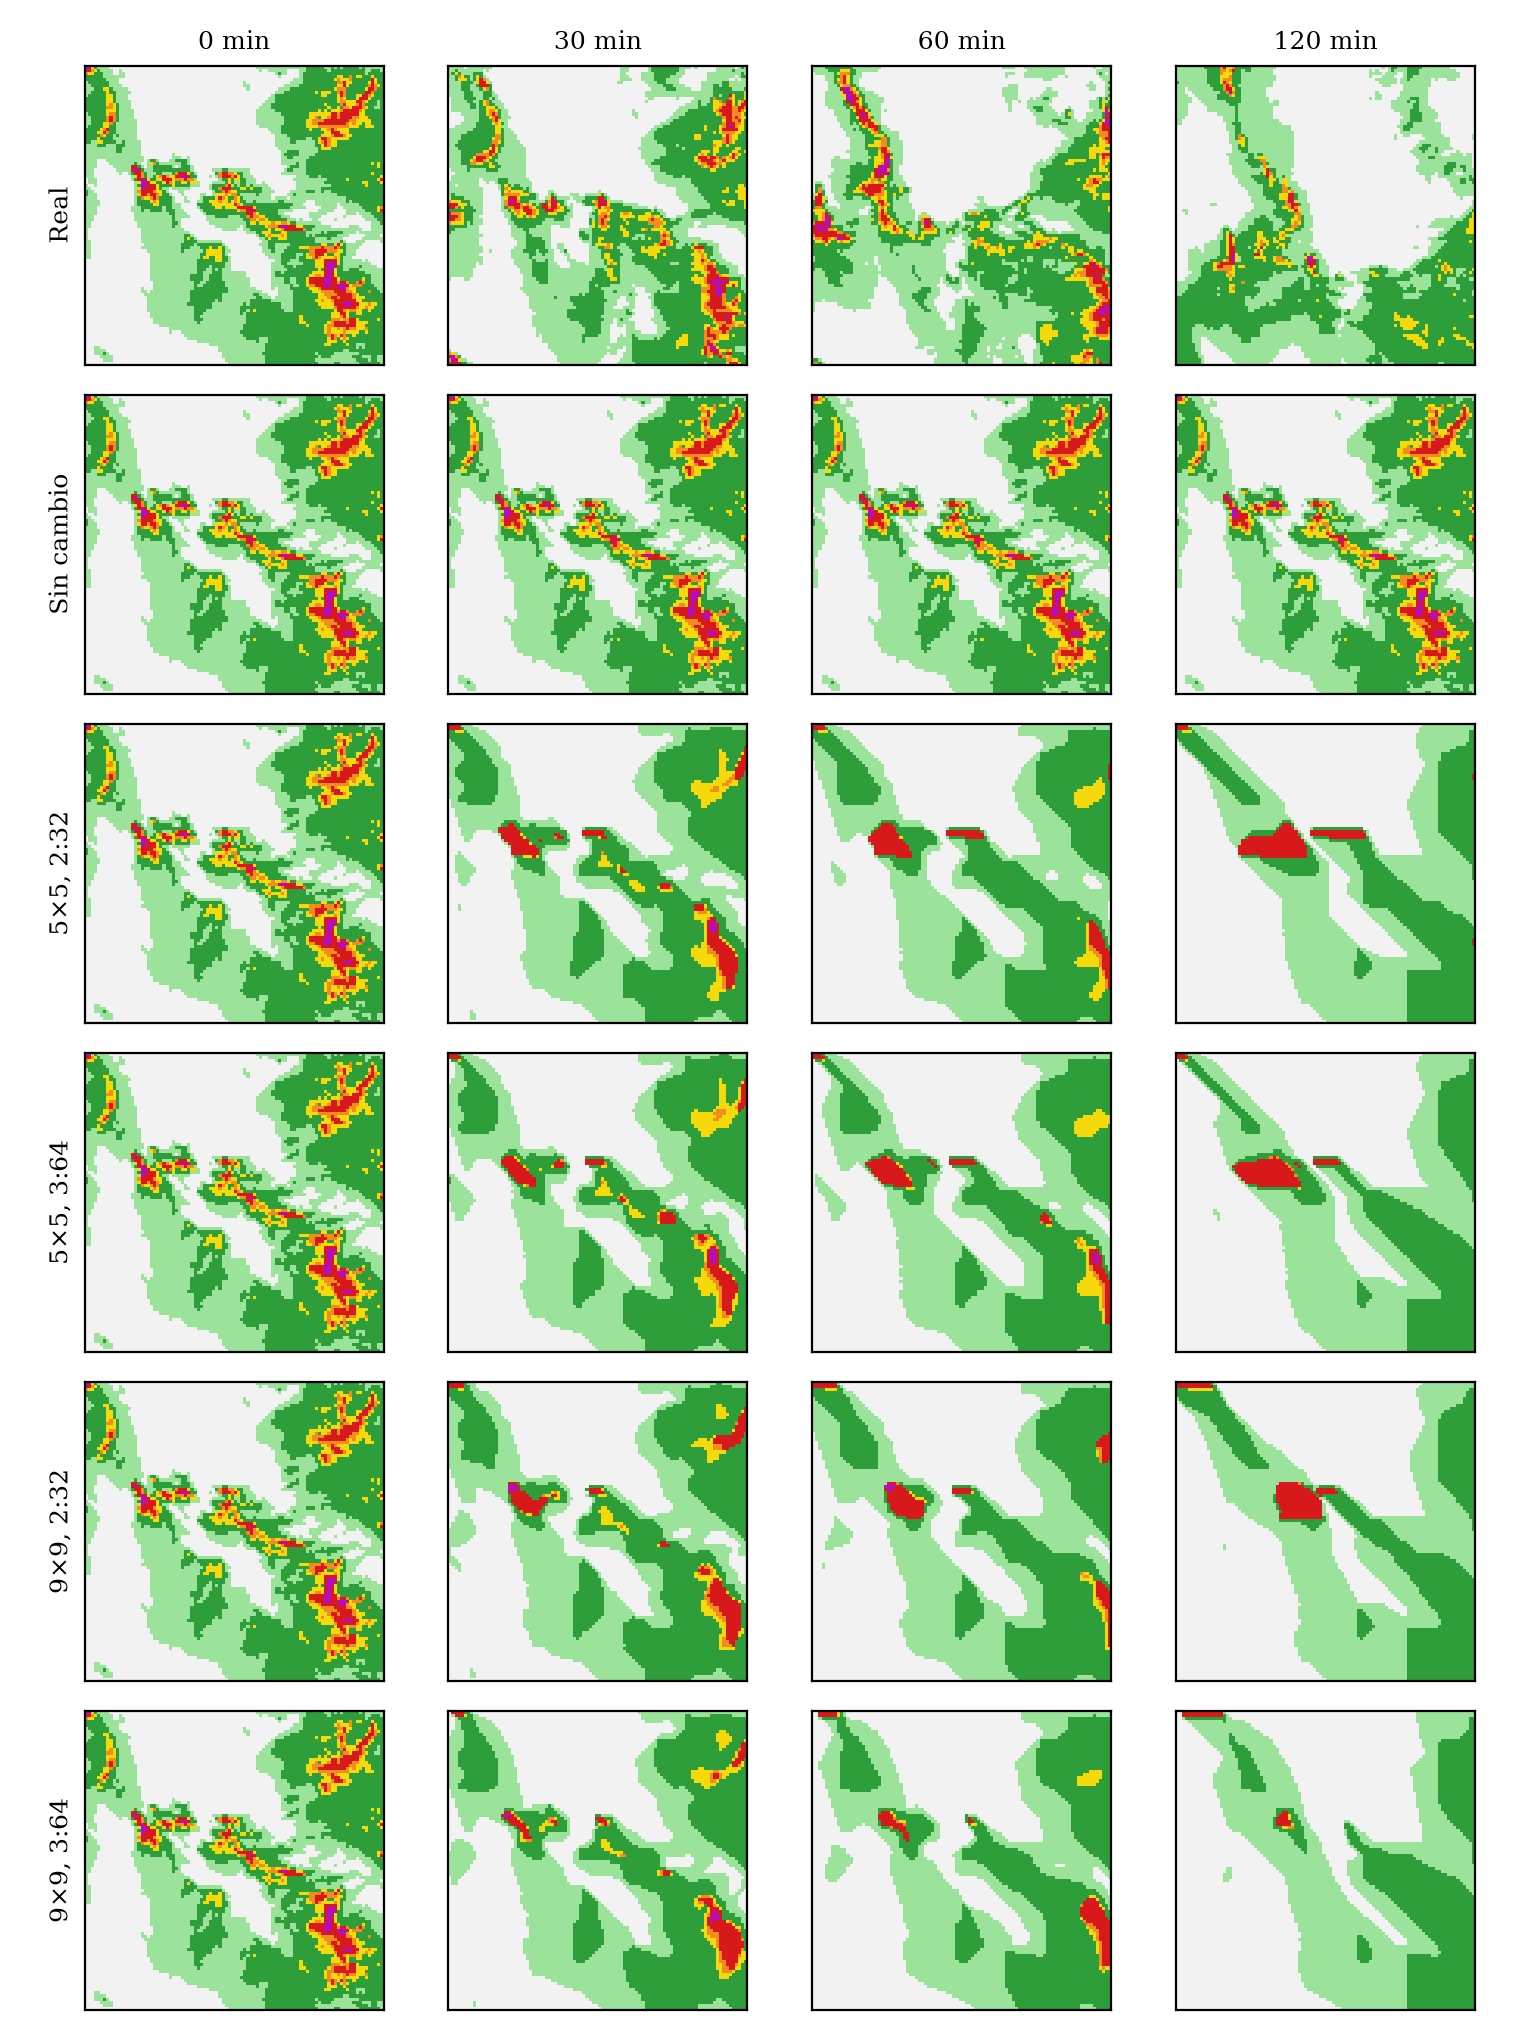
\includegraphics[width=0.8\linewidth]{img/experimentacion/naturales/SEVIR/comparacion.png}
	\leyendasevir
	\caption{Evolución real de la tormenta de la figura \ref{fig:sevir_preprocesamiento}, predicción sin cambio y simulación libre de las 4 configuraciones a los 0, 30, 60 y 120 minutos.}
	\label{fig:sevir_comparacion}
\end{figure}

Esto también se observa en la figura \ref{fig:sevir_area}: en las tormentas de prueba, el área con tormenta real crece del 12.3 al 19.7\% del espacio durante las 4 horas, mientras que en la simulación libre de todas las redes se reduce hasta un 9 o 10\%. Es decir, las redes aprendieron a mover y a debilitar las tormentas, pero no a formarlas ni a intensificarlas.

\begin{figure}[htbp]
	\centering
	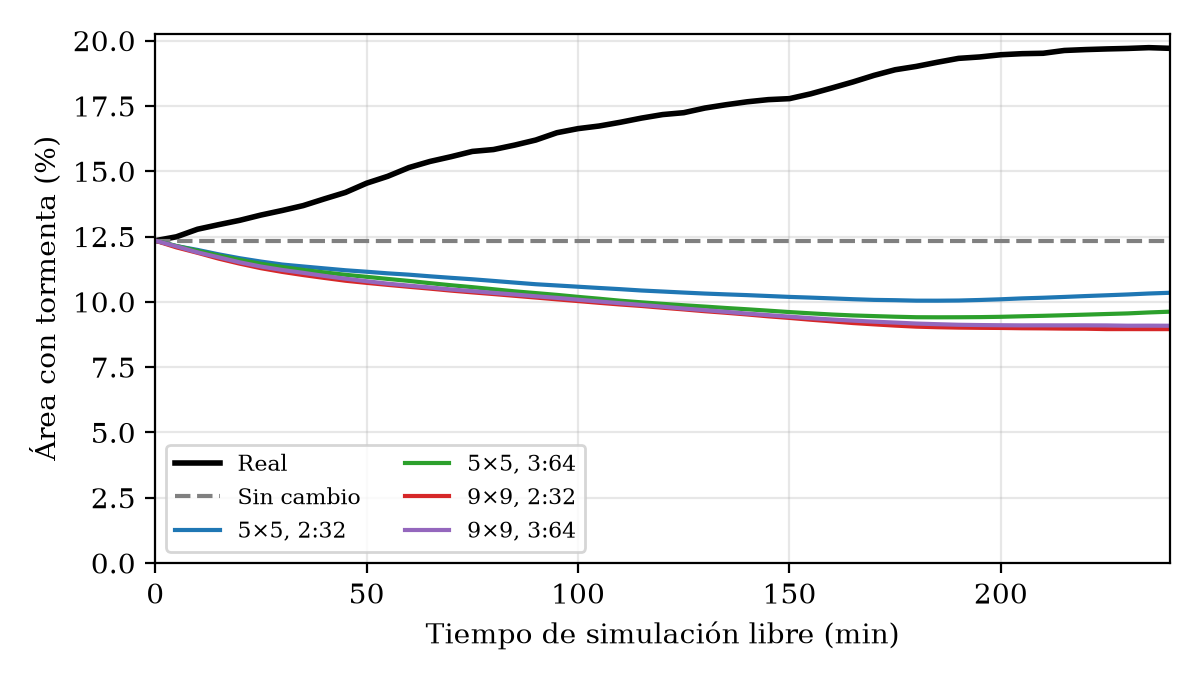
\includegraphics[width=0.75\linewidth]{img/experimentacion/naturales/SEVIR/area.png}
	\caption{Porcentaje del espacio con tormenta (estado 2 o mayor) durante la simulación libre, promedio de las 20 tormentas de prueba.}
	\label{fig:sevir_area}
\end{figure}

Este comportamiento tiene una explicación: cuando la red no puede saber si una célula va a llover más o menos, elige el estado más probable según los datos de entrenamiento, que casi siempre es uno de menos lluvia. Paso a paso, esta elección borra los detalles y debilita las tormentas. Al igual que en FLAME~3, la dinámica depende de variables que no están en las imágenes, como la temperatura, la humedad o el viento a distintas alturas, por lo que la vecindad no contiene toda la información necesaria para predecir el siguiente paso.

\subsubsection{Barrido de configuraciones}

Para saber si el resultado anterior se debe a la poca cantidad de datos o a la configuración de la red, se realizó un barrido con más tormentas, redes más grandes y más vecindades. Se utilizaron las 1,996 tormentas que cumplen la condición de selección para entrenar (1,286 de 2018 y 710 de 2017) y 200 tormentas de 2019 para la prueba, entre las que están las 20 del experimento anterior. Los 7 estados no cambian.

El programa de entrenamiento guarda en memoria la vecindad de cada célula de cada paso, por lo que 40 tormentas completas con la vecindad de $11 \times 11$ ya ocupan cerca de 9 GB. Para usar más tormentas sin rebasar ese límite, de cada tormenta se toman solo algunas transiciones, es decir, pares de imágenes consecutivas, elegidas al azar.

Todas las redes se entrenaron igual que en el experimento anterior (30 épocas, entropía cruzada, tasa de aprendizaje de 0.001 a 0.00001 con reducción exponencial, lote de 8,192 y semilla aleatoria 42) y con frontera abierta: fuera del espacio todas las células están en el estado 0. Una tormenta que entra desde el borde no está en la imagen anterior, por lo que con una frontera periódica la red aprendería que las tormentas aparecen de la nada.

Se probaron 8 vecindades (figura \ref{fig:sevir_vecindades}): 3 cuadradas, 3 circulares y 2 dispersas, la de FLAME~3 y una en forma de estrella, con un núcleo de $5 \times 5$ y 8 rayos que llegan hasta 11 células (44 km) de distancia. Todas tienen como máximo 128 vecinos, por lo que se pueden usar en el simulador. Las capas ocultas fueron 2:32:ReLU, 3:64:ReLU, 8:64:ReLU, 16:64:ReLU y 16:128:ReLU, con capa de salida 7:Linear, y la entrada fue lineal (el estado de cada vecino como un número) o con \textit{one-hot}.

\begin{figure}[htbp]
	\centering
	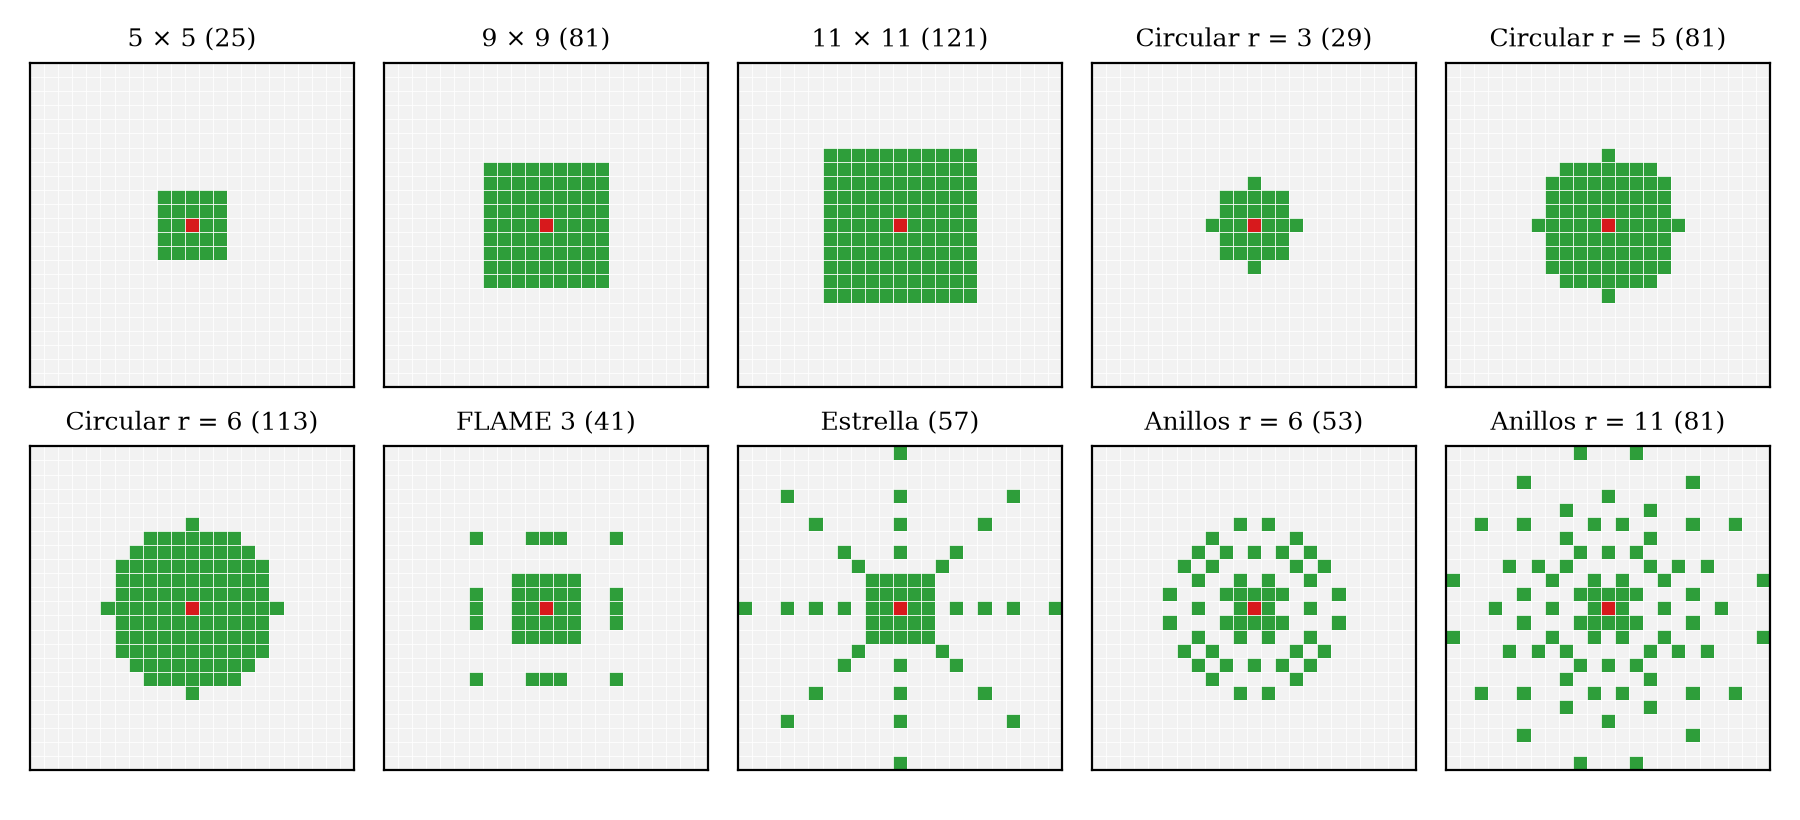
\includegraphics[width=\linewidth]{img/experimentacion/naturales/SEVIR/barrido_vecindades.png}
	\caption{Vecindades probadas en SEVIR y su número de vecinos. En rojo, la célula central. Las de anillos se probaron después del barrido.}
	\label{fig:sevir_vecindades}
\end{figure}

El barrido se dividió en tres fases:

\begin{enumerate}
	\item Pruebas pequeñas: las 80 combinaciones de vecindad, capas ocultas y entrada, con las mismas 40 tormentas completas del experimento anterior. Se eligieron las 4 mejores según el área con tormenta en un paso y en la simulación libre a los 60 y 120 minutos, y según qué tan parecida es la cantidad de tormenta simulada a la real a los 120 minutos.
	\item Más tormentas: las 4 mejores se entrenaron con 400 tormentas de 5 transiciones cada una (casi el mismo número de transiciones que con 40 tormentas completas, pero más variadas) y con 1,000 tormentas de 2 o 3 transiciones.
	\item Estabilidad: la mejor configuración se entrenó con las semillas aleatorias 1 y 2, con 100 épocas y con 4 estados en lugar de 7.
\end{enumerate}

La tabla \ref{tab:sevir_barrido_vecindad} muestra el promedio de las 10 redes de cada vecindad en la primera fase. Las 80 redes superan a la predicción sin cambio en todas las medidas, pero quedan muy cerca unas de otras: el área con tormenta en un paso va de 81.95 a 82.40\% y en la simulación libre a los 60 minutos, de 39.63 a 41.57\%. Las vecindades que llegan a 4 o más células de distancia ($9 \times 9$, $11 \times 11$, circulares de radio 5 y 6, y la de FLAME~3) son un poco mejores que las que llegan a 2 o 3 células. La vecindad de FLAME~3 da casi el mismo resultado que la de $11 \times 11$ con la tercera parte de los vecinos.

\begin{table}[htbp]
	\centering
	\footnotesize
	\setlength{\tabcolsep}{4pt}
	\resizebox{\linewidth}{!}{%
	\begin{tabular}{@{}cccccccc@{}}
		\toprule
		& & & \multicolumn{2}{c}{\textbf{Un paso}} & \multicolumn{2}{c}{\textbf{Área con tormenta en}} & \textbf{Tormenta simulada} \\
		\cmidrule(lr){4-5}
		& & & & \textbf{Área con} & \multicolumn{2}{c}{\textbf{la simulación libre}} & \textbf{respecto a la real} \\
		\cmidrule(lr){6-7}
		\textbf{Vecindad} & \textbf{Vecinos} & \textbf{Pérdida} & \textbf{Exactitud} & \textbf{tormenta} & \textbf{60 min} & \textbf{120 min} & \textbf{a los 120 min} \\ \midrule
		\multicolumn{3}{c}{Predicción sin cambio} & 87.79\% & 77.98\% & 31.78\% & 20.02\% & -- \\ \midrule
		$5 \times 5$ & 25 & 0.2261 & 90.13\% & 82.20\% & 40.02\% & 26.79\% & 65.25\% \\
		$9 \times 9$ & 81 & 0.2215 & 90.17\% & 82.28\% & 40.73\% & 27.95\% & 68.56\% \\
		$11 \times 11$ & 121 & 0.2199 & 90.16\% & 82.26\% & 40.94\% & 28.33\% & 70.22\% \\
		Circular, radio 3 & 29 & 0.2251 & 90.14\% & 82.22\% & 40.25\% & 27.08\% & 66.47\% \\
		Circular, radio 5 & 81 & 0.2214 & 90.17\% & 82.26\% & 40.89\% & 28.27\% & 70.91\% \\
		Circular, radio 6 & 113 & 0.2204 & 90.17\% & 82.28\% & 40.90\% & 28.06\% & 69.37\% \\
		FLAME~3 & 41 & 0.2221 & 90.17\% & 82.28\% & 40.85\% & 28.00\% & 67.99\% \\
		Estrella & 57 & 0.2196 & 90.15\% & 82.25\% & 40.57\% & 27.89\% & 64.99\% \\
		\bottomrule
	\end{tabular}}
	\caption{Primera fase del barrido: promedio de las 10 redes de cada vecindad (5 tamaños de capas ocultas, entrada lineal y \textit{one-hot}), entrenadas con 40 tormentas de 2018 y probadas en 200 tormentas de 2019.}
	\label{tab:sevir_barrido_vecindad}
\end{table}

El tamaño de la red tiene un efecto todavía menor (tabla \ref{tab:sevir_barrido_capas}): pasar de 2:32:ReLU a 16:128:ReLU reduce la pérdida, pero el área con tormenta a los 60 minutos solo sube de 40.34 a 40.83\%, mientras que el tiempo de entrenamiento crece de 35 a 89 segundos. La entrada lineal y el \textit{one-hot} dan prácticamente el mismo resultado (40.74 y 40.55\% a los 60 minutos), y las 4 mejores redes usan entrada lineal: circular de radio 5 con 16:128:ReLU, $11 \times 11$ con 16:64:ReLU, circular de radio 6 con 16:128:ReLU y $11 \times 11$ con 16:128:ReLU.

\begin{table}[htbp]
	\centering
	\footnotesize
	\begin{tabular}{@{}ccccccc@{}}
		\toprule
		& & & \multicolumn{2}{c}{\textbf{Un paso}} & \multicolumn{2}{c}{\textbf{Área con tormenta en}} \\
		\cmidrule(lr){4-5}
		& & \textbf{Tiempo} & & \textbf{Área con} & \multicolumn{2}{c}{\textbf{la simulación libre}} \\
		\cmidrule(l){6-7}
		\textbf{Capas} & \textbf{Pérdida} & \textbf{(s)} & \textbf{Exactitud} & \textbf{tormenta} & \textbf{60 min} & \textbf{120 min} \\ \midrule
		2:32 & 0.2275 & 34.7 & 90.11\% & 82.15\% & 40.34\% & 27.47\% \\
		3:64 & 0.2225 & 37.8 & 90.17\% & 82.24\% & 40.63\% & 27.84\% \\
		8:64 & 0.2210 & 54.5 & 90.18\% & 82.27\% & 40.65\% & 27.76\% \\
		16:64 & 0.2213 & 81.1 & 90.18\% & 82.33\% & 40.78\% & 27.95\% \\
		16:128 & 0.2179 & 88.9 & 90.15\% & 82.28\% & 40.83\% & 27.98\% \\
		\bottomrule
	\end{tabular}
	\caption{Primera fase del barrido: promedio de las 16 redes de cada tamaño de capas ocultas (8 vecindades, entrada lineal y \textit{one-hot}).}
	\label{tab:sevir_barrido_capas}
\end{table}

En la segunda fase (tabla \ref{tab:sevir_barrido_tormentas}), las 4 redes mejoran un poco al pasar de 40 tormentas completas a 400 tormentas con 5 transiciones cada una, aunque el número de transiciones es casi el mismo, es decir, la variedad de tormentas ayuda más que la cantidad de imágenes de cada una. En cambio, con 1,000 tormentas de solo 2 o 3 transiciones los resultados empeoran. La mejor configuración del barrido es la vecindad de $11 \times 11$ con 16:64:ReLU y entrada lineal, entrenada con 400 tormentas.

\begin{table}[htbp]
	\centering
	\footnotesize
	\setlength{\tabcolsep}{4pt}
	\begin{tabular}{@{}cccccccc@{}}
		\toprule
		& & & \textbf{Transiciones} & \textbf{Un paso} & \multicolumn{3}{c}{\textbf{Área con tormenta en}} \\
		& & & \textbf{por} & \textbf{Área con} & \multicolumn{3}{c}{\textbf{la simulación libre}} \\
		\cmidrule(l){6-8}
		\textbf{Vecindad} & \textbf{Capas} & \textbf{Tormentas} & \textbf{tormenta} & \textbf{tormenta} & \textbf{60 min} & \textbf{120 min} & \textbf{240 min} \\ \midrule
		\multicolumn{4}{c}{Predicción sin cambio} & 77.98\% & 31.78\% & 20.02\% & 10.78\% \\ \midrule
		\multirow{4}{*}{Circular, radio 5} & \multirow{4}{*}{16:128} & 40 & 48 & 82.34\% & 41.57\% & 29.20\% & 17.07\% \\
		& & 400 & 5 & 82.65\% & 41.67\% & 28.41\% & 15.66\% \\
		& & 400 & 7 & 82.59\% & 41.31\% & 28.04\% & 15.62\% \\
		& & 1,000 & 3 & 82.62\% & 41.52\% & 28.44\% & 15.82\% \\ \midrule
		\multirow{3}{*}{$11 \times 11$} & \multirow{3}{*}{16:64} & 40 & 48 & 82.36\% & 41.23\% & 28.43\% & 16.55\% \\
		& & 400 & 5 & \textbf{82.67\%} & \textbf{41.83\%} & \textbf{28.84\%} & 16.08\% \\
		& & 1,000 & 2 & 82.55\% & 40.49\% & 27.13\% & 14.17\% \\ \midrule
		\multirow{3}{*}{Circular, radio 6} & \multirow{3}{*}{16:128} & 40 & 48 & 82.40\% & 41.42\% & 28.44\% & 15.85\% \\
		& & 400 & 5 & 82.66\% & 41.68\% & 28.24\% & 15.15\% \\
		& & 1,000 & 2 & 82.56\% & 40.31\% & 26.82\% & 14.34\% \\ \midrule
		\multirow{3}{*}{$11 \times 11$} & \multirow{3}{*}{16:128} & 40 & 48 & 82.34\% & 41.38\% & 28.76\% & 16.88\% \\
		& & 400 & 5 & \textbf{82.67\%} & 41.68\% & 28.18\% & 15.51\% \\
		& & 1,000 & 2 & 82.57\% & 40.23\% & 26.82\% & 14.16\% \\
		\bottomrule
	\end{tabular}
	\caption{Segunda fase del barrido: las 4 mejores redes de la primera fase (entrada lineal) entrenadas con más tormentas. Con 48 transiciones se usa la tormenta completa. Con la vecindad circular de radio 5 caben 7 transiciones de 400 tormentas y 3 de 1,000; con las demás, solo 5 y 2.}
	\label{tab:sevir_barrido_tormentas}
\end{table}

En la tercera fase (tabla \ref{tab:sevir_barrido_estabilidad}), las semillas aleatorias 1 y 2 dan resultados casi iguales a los de la semilla 42, aunque el área con tormenta a los 60 minutos varía hasta 0.8\%, que es más que la diferencia entre muchas de las configuraciones de la primera fase. Entrenar 100 épocas reduce la pérdida, pero no mejora la simulación libre. Con 4 estados (sin lluvia, lluvia, tormenta y tormenta intensa) la red conserva un poco más de tormenta, aunque su exactitud no se puede comparar con la de 7 estados, porque con menos estados es más fácil acertar.

\begin{table}[htbp]
	\centering
	\footnotesize
	\setlength{\tabcolsep}{4pt}
	\begin{tabular}{@{}ccccccc@{}}
		\toprule
		& & \multicolumn{2}{c}{\textbf{Un paso}} & \multicolumn{2}{c}{\textbf{Área con tormenta en}} & \textbf{Tormenta simulada} \\
		\cmidrule(lr){3-4}
		& & & \textbf{Área con} & \multicolumn{2}{c}{\textbf{la simulación libre}} & \textbf{respecto a la real} \\
		\cmidrule(lr){5-6}
		\textbf{Prueba} & \textbf{Pérdida} & \textbf{Exactitud} & \textbf{tormenta} & \textbf{60 min} & \textbf{120 min} & \textbf{a los 120 min} \\ \midrule
		Semilla 42 & 0.2272 & 90.34\% & 82.67\% & 41.83\% & 28.84\% & 70.95\% \\
		Semilla 1 & 0.2277 & 90.35\% & 82.63\% & 41.19\% & 27.56\% & 66.49\% \\
		Semilla 2 & 0.2282 & 90.33\% & 82.63\% & 41.02\% & 27.41\% & 65.16\% \\
		100 épocas & 0.2250 & 90.36\% & 82.53\% & 40.70\% & 27.08\% & 62.45\% \\
		4 estados & 0.1798 & 92.36\% & 82.58\% & 42.24\% & 29.27\% & 76.76\% \\
		\bottomrule
	\end{tabular}
	\caption{Tercera fase del barrido: vecindad de $11 \times 11$, 16:64:ReLU, entrada lineal y 400 tormentas de 5 transiciones. Con 4 estados, la predicción sin cambio tiene una exactitud de 90.26\%; su área con tormenta es la misma que con 7 estados, porque la tormenta sigue siendo el VIL de al menos 74.}
	\label{tab:sevir_barrido_estabilidad}
\end{table}

\subsubsection{Vecindades de anillos}

Por último, se probaron dos vecindades dispersas circulares formadas por anillos (figura \ref{fig:sevir_vecindades}), con la configuración de la mejor red: la célula central, el anillo de radio 1 completo y anillos con 12 a 20 puntos repartidos a la misma distancia. La primera llega a 6 células de distancia con 53 vecinos y la segunda, a 11 células con 81 vecinos. Cada una se entrenó con las semillas aleatorias 42, 1 y 2.

La tabla \ref{tab:sevir_anillos} muestra que ambas dan prácticamente el mismo resultado que la vecindad de $11 \times 11$, con menos de la mitad de los vecinos en el caso de la de radio 6. Ver más lejos no mejora la simulación libre: la vecindad de radio 11 tiene el área con tormenta en un paso más alta y la menor variación entre semillas, pero conserva un poco menos de tormenta.

\begin{table}[htbp]
	\centering
	\footnotesize
	\setlength{\tabcolsep}{4pt}
	\begin{tabular}{@{}cccccccc@{}}
		\toprule
		& & \multicolumn{2}{c}{\textbf{Un paso}} & \multicolumn{3}{c}{\textbf{Área con tormenta en}} & \textbf{Tormenta simulada} \\
		\cmidrule(lr){3-4}
		& & & \textbf{Área con} & \multicolumn{3}{c}{\textbf{la simulación libre}} & \textbf{respecto a la real} \\
		\cmidrule(lr){5-7}
		\textbf{Vecindad} & \textbf{Vecinos} & \textbf{Exactitud} & \textbf{tormenta} & \textbf{60 min} & \textbf{120 min} & \textbf{240 min} & \textbf{a los 120 min} \\ \midrule
		\multicolumn{2}{c}{Predicción sin cambio} & 87.79\% & 77.98\% & 31.78\% & 20.02\% & 10.78\% & -- \\ \midrule
		$11 \times 11$ & 121 & 90.34\% & 82.64\% & 41.35\% & 27.93\% & 15.14\% & 67.53\% \\
		Anillos, radio 6 & 53 & 90.31\% & 82.59\% & 41.18\% & 27.61\% & 14.77\% & 65.99\% \\
		Anillos, radio 11 & 81 & 90.36\% & 82.68\% & 41.24\% & 27.69\% & 14.73\% & 64.49\% \\
		\bottomrule
	\end{tabular}
	\caption{Vecindades de anillos contra la de $11 \times 11$, con 16:64:ReLU, entrada lineal y 400 tormentas de 5 transiciones. Promedio de las semillas aleatorias 42, 1 y 2.}
	\label{tab:sevir_anillos}
\end{table}

Las figuras \ref{fig:sevir_barrido_comparacion} y \ref{fig:sevir_barrido_area} muestran que el comportamiento del experimento anterior no cambia con más tormentas ni con otras vecindades. Las redes conservan la forma general y la dirección de las tormentas, pero las convierten en manchas uniformes, y el área con tormenta de la simulación libre se queda entre el 11 y el 12\% del espacio, mientras que la real crece del 12.6 al 17.6\%.

\begin{figure}[htbp]
	\centering
	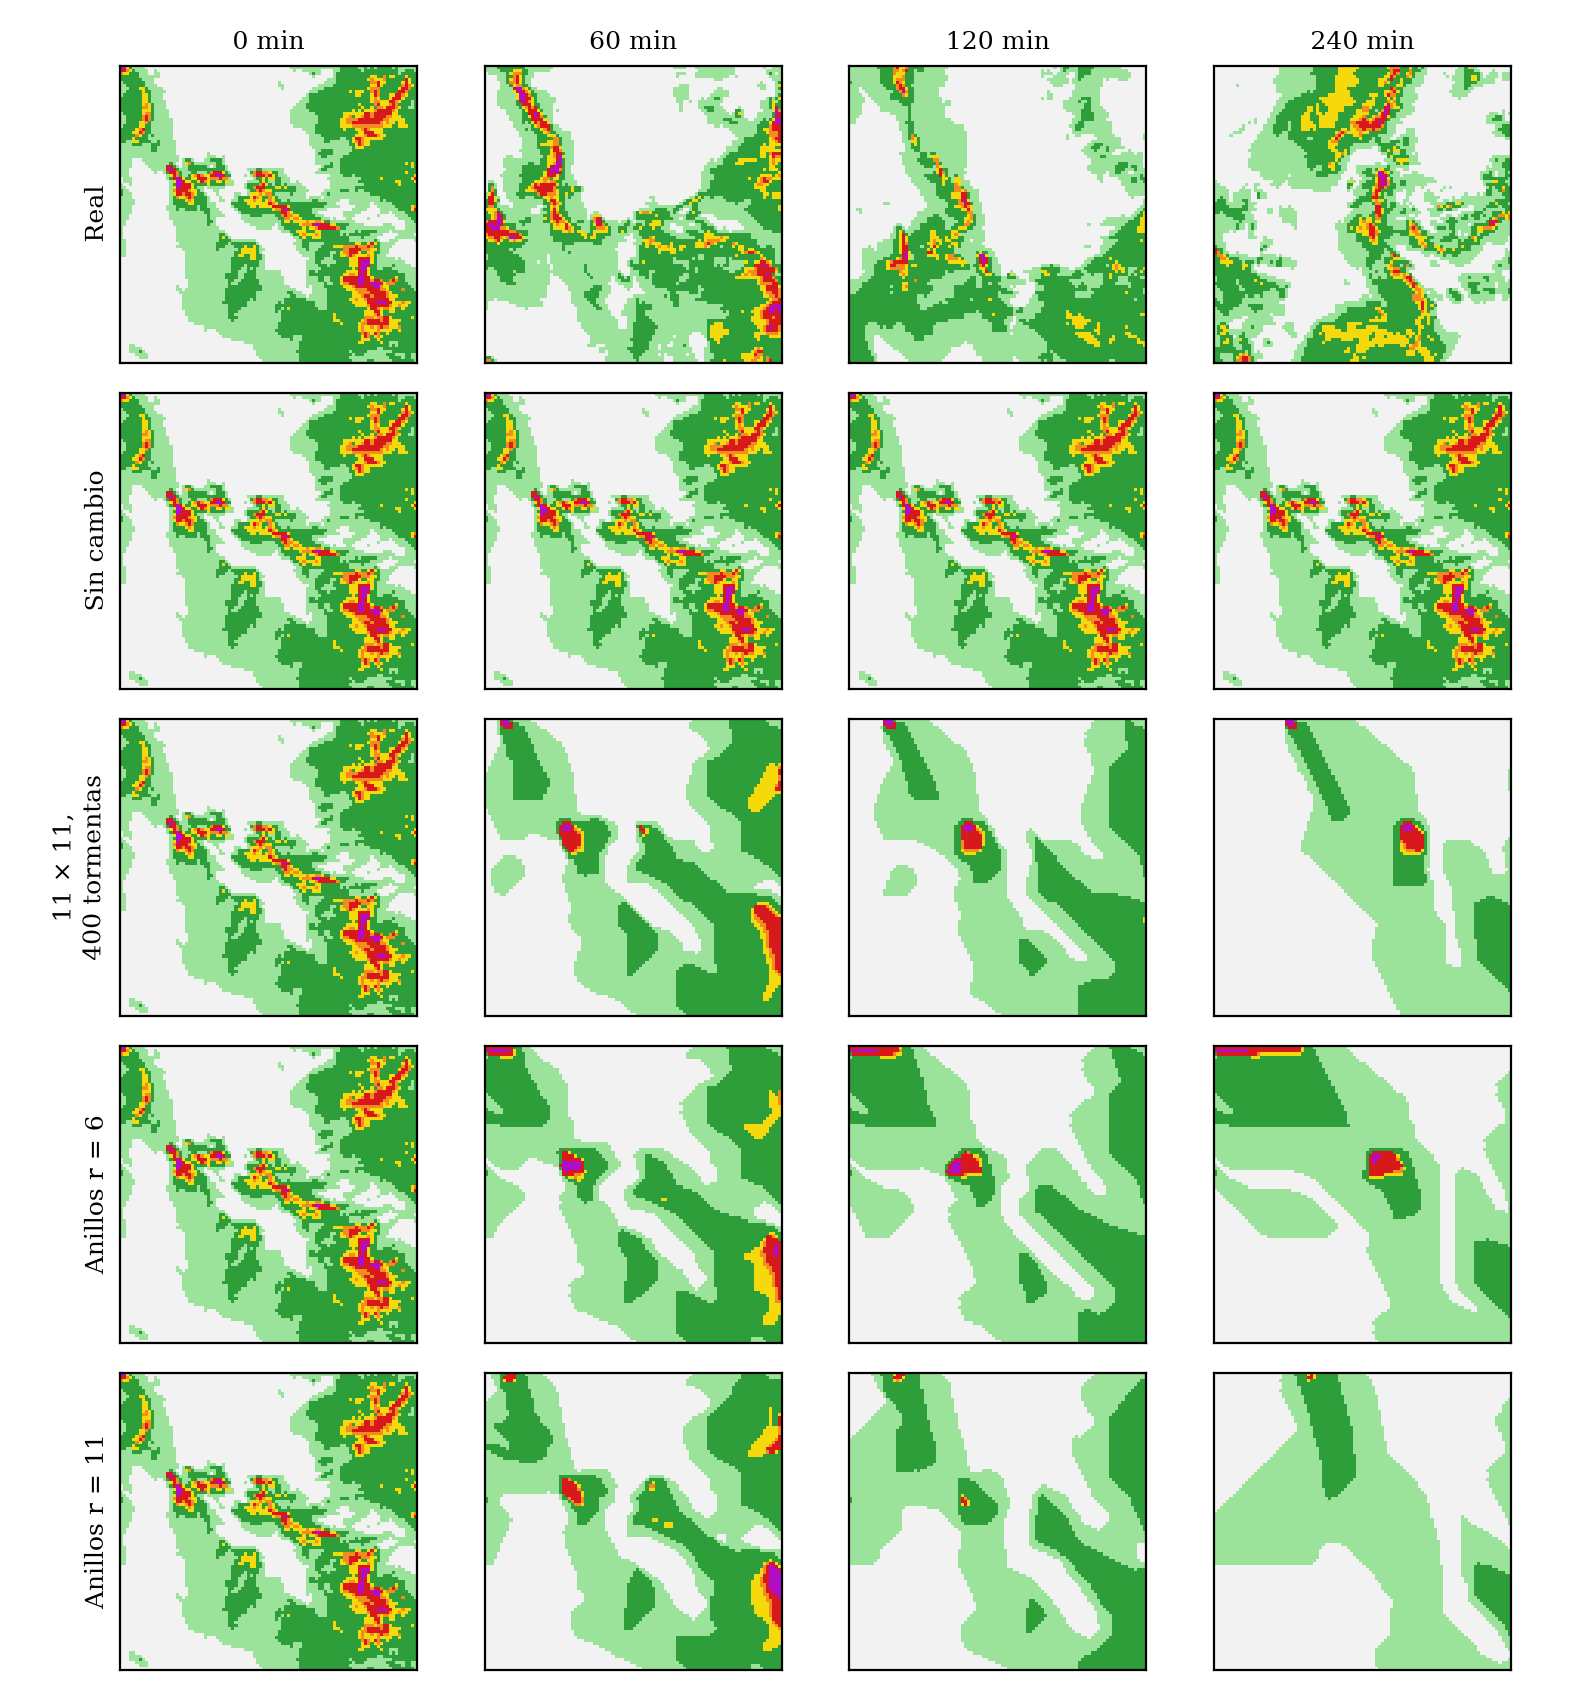
\includegraphics[width=0.8\linewidth]{img/experimentacion/naturales/SEVIR/barrido_comparacion.png}
	\leyendasevir
	\caption{Evolución real de la tormenta de la figura \ref{fig:sevir_preprocesamiento}, predicción sin cambio y simulación libre de la mejor red del barrido ($11 \times 11$) y de las vecindades de anillos, todas con 16:64:ReLU y 400 tormentas, a los 0, 60, 120 y 240 minutos.}
	\label{fig:sevir_barrido_comparacion}
\end{figure}

\begin{figure}[htbp]
	\centering
	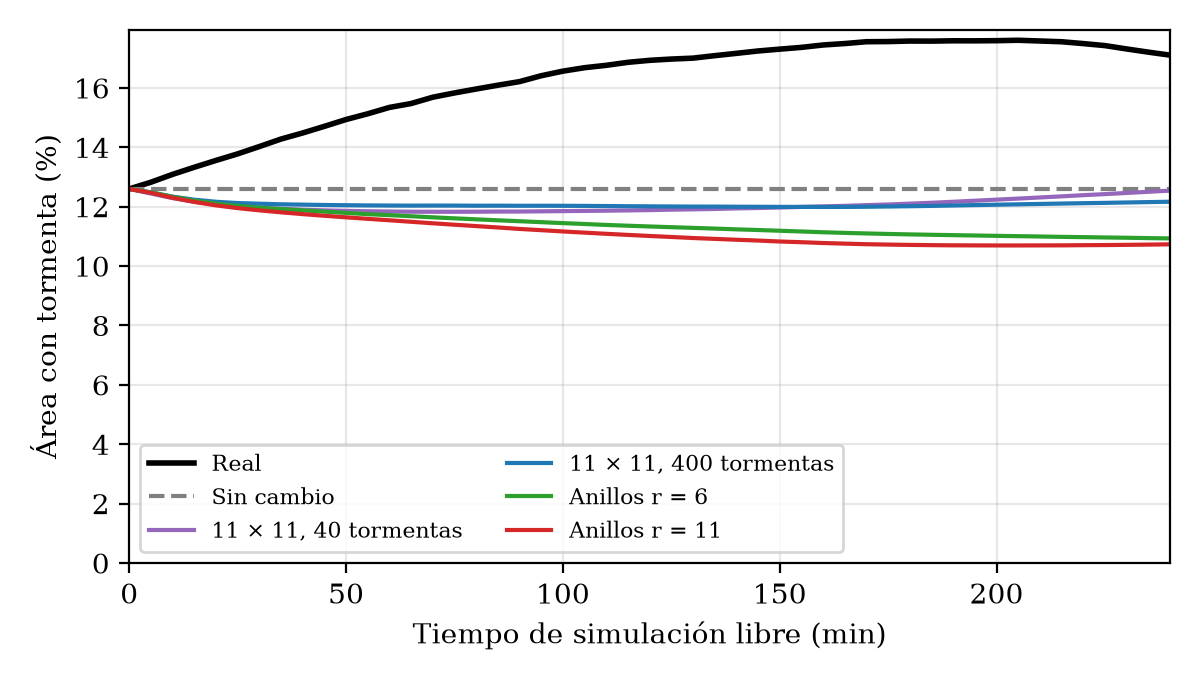
\includegraphics[width=0.75\linewidth]{img/experimentacion/naturales/SEVIR/barrido_area.png}
	\caption{Porcentaje del espacio con tormenta (estado 2 o mayor) durante la simulación libre, promedio de las 200 tormentas de prueba. Todas las redes usan 16:64:ReLU y entrada lineal.}
	\label{fig:sevir_barrido_area}
\end{figure}

\subsubsection{Desplazamiento de las tormentas}

Para saber qué aprendió la red, se midió cuánto se desplaza cada tormenta en 60 minutos, buscando el corrimiento de la primera imagen que mejor coincide con las células con tormenta a los 60 minutos. La tabla \ref{tab:sevir_desplazamiento} muestra que la red mueve casi todas las tormentas hacia el este, que es la dirección más común en los Estados Unidos, con mucha menos variación que las tormentas reales. La relación entre el desplazamiento de la red y el real es débil: la red se equivoca en promedio por unas 5 células, mientras que mover todas las tormentas con el desplazamiento promedio se equivoca por unas 6.

\begin{table}[htbp]
	\centering
	\footnotesize
	\begin{tabular}{@{}cccc@{}}
		\toprule
		& \textbf{Desplazamiento promedio} & \textbf{Variación entre tormentas} & \textbf{Relación con el real} \\
		& \textbf{hacia el este} & \textbf{(este--oeste / norte--sur)} & \textbf{(este--oeste / norte--sur)} \\ \midrule
		Real & 5.82 células (23 km) & 7.06 / 7.18 células & -- \\
		Red & 7.17 células (29 km) & 4.49 / 4.04 células & 0.36 / 0.51 \\
		\bottomrule
	\end{tabular}
	\caption{Desplazamiento de las células con tormenta en 60 minutos en las 200 tormentas de prueba, real y en la simulación libre de la mejor red ($11 \times 11$, 16:64:ReLU, 400 tormentas). La variación es la desviación estándar y la relación es la correlación entre el desplazamiento de la red y el real (1 sería idéntico).}
	\label{tab:sevir_desplazamiento}
\end{table}

Es decir, la red aprendió principalmente a desplazar las tormentas. La dirección en la que se mueve una tormenta depende del viento, que no está en las imágenes de VIL, y lo mismo ocurre con su crecimiento, que depende de la humedad y la temperatura del aire, y con las tormentas que entran desde fuera del espacio. Dos tormentas con la misma imagen pueden moverse en direcciones distintas, por lo que la vecindad no tiene la información necesaria para predecir el siguiente paso. Un autómata celular es un sistema cerrado, en el que la evolución depende solo de los estados de las células, y las tormentas no cumplen esa condición.

De este experimento podemos concluir que el autómata celular neuronal sí aprende parte de la dinámica de las tormentas a partir de su evolución, ya que supera a la predicción sin cambio en tormentas de un año que nunca vio. Sin embargo, con 7 estados y una sola variable, la simulación libre pierde las tormentas en pocas horas. El barrido muestra que este límite no depende de la cantidad de datos, del tamaño de la red ni de la vecindad, sino de que las tormentas son un sistema abierto, que depende de factores externos como el viento.
